% \documentclass[10pt,twocolumn,oneside]{article}
\documentclass[12pt,onecolumn,oneside]{article}
% \usepackage{simpleConference}
\usepackage{times}
\usepackage{graphicx}
\usepackage{colortbl}
\usepackage{todonotes}
\usepackage{url,hyperref}
\hypersetup{colorlinks=true, linkcolor=blue}
\usepackage{fancyvrb}
\usepackage{verbatim}
\usepackage[top=1in, bottom=1in, left=1.5in, right=1in]{geometry}
\usepackage{fixltx2e}
% Install package: texlive-science
\usepackage{algorithmic} 
% singlelinecheck (false) - Remove some of the space between figure and caption
% skip = 0pt
% Install package: texlive-generic-extra
\usepackage[font=small,labelfont=bf, singlelinecheck=false, skip=0pt]{caption}
\usepackage{subcaption}


%Remove hyphens
\usepackage[none]{hyphenat}

\begin{document}
% Turn of page numbering for now
\pagenumbering{gobble}
\title{System-wide Performance Analysis for Virtualization}
\author{Deron Jensen\\
\\
Department of Computer Science\\
Portland State University\\
Portland, OR \\
deron@cs.pdx.edu \\
}
\date{\today}
% \onecolumn[
% \begin{@twocolumnfalse}
  \maketitle
\newpage

\begin{abstract}
With the current trend in cloud computing and virtualization, more organizations are moving their systems from a physical host to a virtual server.  Although this can significanlty reduce hardware, power, and administration costs, it can increase cost in analyzing performance problems.  With virtualization, there is an initial performance overhead, and as more virtual machines are added to a physical host the interference increases between various guest machines.  When this interference occurs, a virtualized guest application may not perform as expected.  Additionally, there is little or no information to the virtual OS about the interference.  From the hypervisor viewpoint, tools are available to view each virtual machine, but the interference is not available. \newline
\indent  We examine the interference that has been shown in previous research, and relate that to existing tools and research in root cause analysis.  We show that in virtualization there are addtional layers which need to be analyzed, and design a framework to determine if degradation is occuring from an external virtualization layer.  Additionally, we build a virtualization test suite with Xen and PostgreSQL and run multiple tests to create I/O interference.  We show how our framework can determine if the problem is from external interference when an application is degraded.   
  \end{abstract}
\newpage
% \end{@twocolumnfalse}

\setcounter{page}{1}
\pagenumbering{arabic}
% 1.  This is a comment
\section{Introduction}
System virtualization is a way for a data center to reduce cost and power by overcommitting and sharing system resources across disparate operating systems with common hardware.  Since each guest machine only uses a portion of the available resources at any given time, the total resources allocated to all guest VMs can exceed the total physical resources \cite{huber2, amit, buell1}.   This idea of overcommitting resources is the same as preemptive multitasking, where multiple processes share a single CPU; and OS virtual memory, where the total memory available to applications exceeds the physical memory capacity.   

\indent Due to these cost savings and lower physical administration overhead, IT Data Centers and Businesses are moving toward virtualized environments.  In 2008 Gartner’s showed that 12\% of hardware at data centers were virtualized, and then predicted that by 2013 61\% would be virtualized \cite{gartners}.   Additionally, research from Ramya and Edwin show tremendous growth in Platform As A Service (PAAS) where an entire system platform is dynamically provisioned in a cloud computing service \cite{ramya}.   Massive data centers are able to provide virtual systems, and manage large clusters of shared resources, while meeting expected Service Level Agreements, for a fraction of the price of building a physical server for each customer.

\begin{figure}[!b]
  \begin{center}
    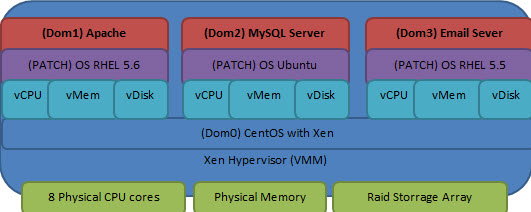
\includegraphics[width=3.5in]{images/VirtualizationExample.jpg}
  \end{center}

  \caption{\small In this example there are 3 paravirtualized guests (DomU) running on a Xen Server.  The Xen hypervisor and Dom0 divide, share, and overcommit the physical resources between the 3 guest domains.  Each guest has access to virtual resources and not physical hardware.}
  \label{fig-VirtualizationExample.pdf}
\end{figure}


\indent The problem this introduces is in performing profiling and analysis of this additional layer of abstraction.  The hypervisor, or Virtual Machine Manager, adds to the already complex existing layers (Application, OS, and Hardware) one must analyze when an application performs sub-optimally.  How can a system administrator determine if the problem is in the application, OS, hypervisor, hardware, or an unrelated guest virtual machine on the same physical host system?  In a traditional environment there can be 'interference' \cite{paul}or ‘system noise' caused by these layers, which attributes to poor application performance.  The hypervisor as well as multiple other guest virtual machines which compete for system resources add to this outside interference, which is undetectable from a guest VM, and therefore undetectable by the guest applications.

\indent This paper we show that using existing profiling tools and measuring changes in system runtime data in the guests and VMM we are now able to determine the layer of the complex software stack that attributes to a sub-optimal running application in a virtual environment.  Additionally, we can determine which system resource (memory, CPU, or IO) needs to be modified or is used inefficiently.

\indent This project will add the following contributions for virtualization:
\begin{enumerate}
\item Define the layers of abstraction in various virtual environments.
\item Define the system resources which attributes to application problem from I/O, memory, or CPU problems.
\item Framework to Identify the counters, metrics, and envirement at each layer which contributes to I/O contention.
\item Example tool which dynamically analyzes runtime interference and identifies the layer which experiences I/O contention.
\item Introduce \emph{disk pinning} for virtualization where separate physical disks are assigned to individual virtual servers.
\end{enumerate}



\newpage

\begin{thebibliography}{9}
\bibitem{huber1}
Huber, Nikolaus, et al. \emph{Analysis of the performance-influencing factors of virtualization platforms.}  On the Move to Meaningful Internet Systems, OTM 2010. Springer Berlin Heidelberg, 2010. 811-828.
\bibitem{huber2}
Huber, Nikolaus, et al. \emph{A Method for Experimental Analysis and Modeling of Virtualization Performance Overhead.}  Cloud Computing and Services Science. Springer New York, 2012. 353-370.
\bibitem{tickoo} 
Tickoo, Omesh, et al.  \emph{Modeling virtual machine performance: challenges and approaches.}  ACM SIGMETRICS Performance Evaluation Review 37.3 (2010): 55-60.
\bibitem{menon} Menon, Aravind, et al.  \emph{Diagnosing performance overheads in the xen virtual machine environment.}  Proceedings of the 1st ACM/USENIX international conference on Virtual execution environments. ACM, 2005.
\bibitem{kundu}Kundu, Sajib, et al.  \emph{Application performance modeling in a virtualized environment.}  High Performance Computer Architecture (HPCA), 2010 IEEE 16th International Symposium on. IEEE, 2010.
\bibitem{cherkasova}
Cherkasova, Ludmila, and Rob Gardner.  \emph{Measuring CPU overhead for I/O processing in the Xen virtual machine monitor.}  Proceedings of the USENIX annual technical conference. 2005.
\bibitem{traeger}
Traeger, Avishay, Ivan Deras, and Erez Zadok.  \emph{DARC: Dynamic analysis of root causes of latency distributions.}  ACM SIGMETRICS Performance Evaluation Review 36.1 (2008): 277-288
\bibitem{knapp1}
Knapp, Rashawn L., Karen L. Karavanic, and Douglas M. Pase.  \emph{Detecting runtime environment interference with parallel application behavior.}  Parallel and Distributed Processing Symposium, 2007. IPDPS 2007. IEEE International. IEEE, 2007.
\bibitem{kprobes}
Kprobes   https://www.kernel.org/doc/Documentation/kprobes.txt
\bibitem{paul}
Paul, Indrani, Sudhakar Yalamanchili, and Lizy K. John.  \emph{Performance impact of virtual machine placement in a datacenter.}  Performance Computing and Communications Conference (IPCCC), 2012 IEEE 31st International. IEEE, 2012.
\bibitem{mucci}
Mucci, Philip J., et al.  \emph{PAPI: A portable interface to hardware performance counters.}  Proc. Department of Defense HPCMP Users Group Conference. 1999.
\bibitem{mohror}
Mohror, Kathryn, and Karen L. Karavanic.  \emph{Towards scalable event tracing for high end systems.}  High Performance Computing and Communications. Springer Berlin Heidelberg, 2007. 695-706.
\bibitem{kufrin}
Kufrin, Rick.  \emph{Perfsuite: An accessible, open source performance analysis environment for linux.}  6th International Conference on Linux Clusters: The HPC Revolution. Vol. 151. 2005.
\bibitem{jafar}
Jafar, Anderson, and Abdullat (2008). \emph{Comparison of Dynamic Web Content Processing Language Performance Under a LAMP Architecture}  Journal of Information Systems Applied Research, 1 (1). \url{http://jisar.org/1/1/. ISSN: 1946-1836.}
\bibitem{saltzer}
Saltzer, Jerome H., David P. Reed, and David D. Clark.  \emph{End-to-end arguments in system design.}  ACM Transactions on Computer Systems (TOCS) 2.4 (1984): 277-288.
\bibitem{katcher}
Katcher, Jeffrey. Postmark: A new file system benchmark. Technical Report TR3022, Network Appliance, 1997. www. netapp. com/tech\_library/3022. html, 1997.
\bibitem{gupta1}
Gupta, Vishakha, Rob Knauerhase, and Karsten Schwan.  \emph{Attaining system performance points: revisiting the end-to-end argument in system design for heterogeneous many-core systems.}  ACM SIGOPS Operating Systems Review 45.1 (2011): 3-10.
\bibitem{levon}
Levon, John, and Philippe Elie.  \emph{Oprofile: A system profiler for linux.}  2012-05-05. \url{http://oprofile, sf. net (2004).}
\bibitem{tikotekar}
Tikotekar, Anand, et al.  \emph{An analysis of hpc benchmarks in virtual machine environments.}  Euro-Par 2008 Workshops-Parallel Processing. Springer Berlin Heidelberg, 2009.
\bibitem{santos}
Santos, Renato J.  “Tutorial:  Profiling in Xen” \url{http://xen.xensource.com/files/summit\_3/xenoprof\_tutorial.pdf}  HP Labs  Xen Summit, 2006
\bibitem{menon2}
Menon, Santos, Yoshio, Janakiraman.  XENOPROF – Performance profiling in Xen.  User Guide.   \url{http://xenoprof.sourceforge.net/xenoprof\_2.0.txt}  2005.
\bibitem{joukov}
Joukov, Nikolai, et al.  \emph{Operating system profiling via latency analysis.}  Proceedings of the 7th symposium on Operating systems design and implementation. USENIX Association, 2006.
\bibitem{gupta2}
Gupta, Vishakha, et al.  \emph{Pegasus: Coordinated scheduling for virtualized accelerator-based systems.}  2011 USENIX Annual Technical Conference (USENIX ATC’11). 2011.
\bibitem{ahmad}
Ahmad, Irfan, Ajay Gulati, and Ali Mashtizadeh.  \emph{vIC: Interrupt coalescing for virtual machine storage device IO.}  USENIX Annual Technical Conference (ATC). 2011.
\bibitem{amit}
Amit, Nadav, et al.  \emph{vIOMMU: efficient IOMMU emulation.}  USENIX Annual Technical Conference (ATC). 2011.
\bibitem{lim}
Lim, Harold, Aman Kansal, and Jie Liu.  \emph{Power budgeting for virtualized data centers.}  2011 USENIX Annual Technical Conference (USENIX ATC’11). 2011.
\bibitem{vmwareMem}
VMware, Inc.  Performance Study.  \emph{Understanding Memory Resource Management in VMware ESX 4.1.} \url{http://www.vmware.com/files/pdf/techpaper/vsp\_41\_perf\_memory\_mgmt.pdf}
\bibitem{boutcher}
Boutcher, David, and Chandra Abhishek. \emph{Does Virtualization Make Disk Scheduling Passé?}  Univerisity of Minnesota.  \url{http://www-users.cs.umn.edu/~chandra/papers/hotstorage09/paper.pdf}
\bibitem{diskeeper}
Diskeeper, Inc.  \emph{Virtualization and Disk Performance}  \url{http://files.diskeeper.com/pdf/virtualization\_performance.pdf}
\bibitem{IBMsar}
IBM, Inc. \emph{Assessing disk performance with the sar command}  \url{http://publib.boulder.ibm.com/infocenter/pseries/v5r3/index.jsp?topic=/com.ibm.aix.prftungd/doc/prftungd/assess\_disk\_perf\_sar.htm}
\bibitem{soundararajan}
Soundararajan, Gokul, and Cristiana Amza.  \emph{Towards end-to-end quality of service: controlling I/O interference in shared storage servers.}  Proceedings of the 9th ACM/IFIP/USENIX International Conference on Middleware. Springer-Verlag New York, Inc., 2008.
\bibitem{lumb}
Lumb, Christopher R., Arif Merchant, and Guillermo A. Alvarez.  \emph{Façade: Virtual storage devices with performance guarantees.}  (2003).
\bibitem{knapp2}
Knapp, Rashawn L., R. L. Pase, and Karen L. Karavanic.  \emph{ARUM: application resource usage monitor.}  9th Linux Clusters Institute International Conference on High-Performance Clustered Computing. 2008.
\bibitem{gartners}
Bittman, Thomas J.  \emph{Server virtualization trends in 2008: Everything changes.}  Gartner Research, March (2008).
\bibitem{ramya}
Catherine, M. Ramya, and E. Bijolin Edwin.  \emph{A Survey on Recent Trends in Cloud Computing and its Application for Multimedia.}  International Journal of Advanced Research in Computer Engineering \& Technology (IJARCET) 2.1 (2013): pp-304.
\bibitem{vmWareIO} 
VMware, Inc. \emph{Storage system performance analysis with IOmeter.}  \url{http://communities.vmware.com/docs/DOC-3961}
\bibitem{suseIO} 
Suse Chapter 13.  \emph{Tuning I/O Performance.}  \url{http://doc.opensuse.org/products/draft/SLES/SLES-tuningsdraft/cha.tuning.io.html}
\bibitem{hplBench} 
\emph{HPL Benchmark: the Linpack TPP benchmark which measures the floating point rate of execution for solving a linear system of equations.}  \url{http://www.netlib.org/benchmark/hpl/}
\bibitem{hpcChallenge} 
\emph{HPC Challenge:}  \url{http://icl.cs.utk.edu/hpcc/}
\bibitem{pgTune} 
Momjian, Bruce. \emph{PostgresSQL Hardware Performance Tuning.}  \url{http://momjian.us/main/writings/pgsql/hw\_performance/}
\bibitem{du1} 
Du, Jiaqing, Nipun Sehrawat, and Willy Zwaenepoel.  \emph{Performance profiling in a virtualized environment.}  Proc. HotCloud (2010).
\bibitem{du2}
Du, Jiaqing, Nipun Sehrawat, and Willy Zwaenepoel.  \emph{Performance profiling of virtual machines.}  ACM SIGPLAN Notices. Vol. 46. No. 7. ACM, 2011.
\bibitem{serebrin}
Serebrin, Benjamin, and Daniel Hecht.  \emph{Virtualizing performance counters.}  Euro-Par 2011: Parallel Processing Workshops. Springer Berlin Heidelberg, 2012.
\bibitem{buell1}
Buell, J., Hecht, D., Heo, J., Saladi, K. and Taheri, H. R.  \emph{Methodology for Performance Analysis of VMware vSphere under Tier-1 Applications.}  VMware Technical Journal Vol 2. No. 1.  June 2013.
\bibitem{buell2} 
Buell, J., Hecht, D., Heo, J., Saladi, K. and Taheri, H. R.  \emph{Overcommitment in the ESX Server.}  VMware Technical Journal Vol 2. No. 1.  June 2013.
\end{thebibliography}
\end{document}


\end{document}
